\chapter{Installation and Use Case} 

This chapter teaches user how to install and use Teakwood. Teakwood is designed for scientific researcher's daily use. A simple and compatible folw logic for submitting jobs is important. Teakwood created a maximally generalized working flow to fit most computing tools. 
Regarding the installation, Teakwood provides a one-execution set up. However, lake of required system components will lead Teakwood malfunctioning. Install system requirements is a necessary.\\

\section{System requirements}

Teakwood is a Django web framework which integrated a lot of third party packages and external tools; some of the packages or tools require extra libs and development packages to work. Before running Teakwood, we need to resolve all those dependencies as well as finish setting up all the packages and tools. Below is a list of the required installations during the Teakwood development.\\

$\bullet$ \textbf{Project Dependent libs}\\
As mentioned above, installing all dependent libs are the first step. Please refer to the installation guide in homepage for more information.\\

$\bullet$ \textbf{MySQL Database}\\
Teakwood uses MySQL database, so make sure mysql-server and mysql-devel is installed. If you want a GUI control of your database, I recommend an installation of phpMyAdmin. \\

$\bullet$ \textbf{Version Control}\\
Git is a very popular version control tool. Teakwood uses git as version control, and  Teakwood source code is hosted in Github.\\

$\bullet$ \textbf{Virtual Environment}\\
It is highly recommended that we set up an independent working environment for Teakwood development. "Virtualenv" is a reliable solution.\\

$\bullet$ \textbf{Latex and Sphinx}\\
Teakwood uses sphinx package to generate diverse types of files such as HTML, Latex, and PDF. Hence, sphinx and Latex need to be installed.\\

$\bullet$ \textbf{Celery and RabbitMQ}\\
This is a solution for resolving synchronous process. install and start them before you run Teakwood.\\

$\bullet$ \textbf{Django 1.4.x}\\
No need to explain. \\

$\bullet$ \textbf{Third Party Packages}\\
Teakwood uses a lot of "wheels" to construct the structure. before runing Teakwood, those wheels need to be installed in the right path. Refer "requirements.txt" for the "wheels" list.

\section{Job Submission}
Let's take a look at the classical job submission flow in Teakwood.
\begin{figure}[h]
\centering
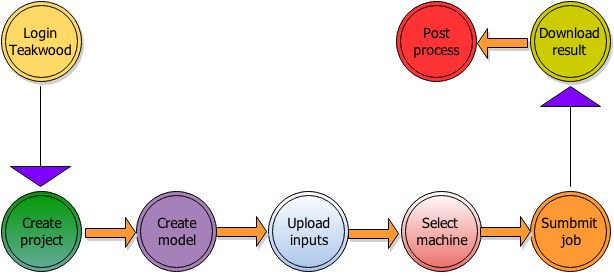
\includegraphics[scale=0.5]{./submission}
\caption{Job Submission Flow}
\label{fig:label} % insert suitable label, this is used to refer to a fig from within the text as shown above
\end{figure}

On the above figure, each circle represents a different stage:\\

$\bullet$ \textbf{Login}: Only logged user can use the working console, visitors only can see the information page. Login is a necessary.\\
$\bullet$ \textbf{Project}: A project relates to a big problem resolving. A project may use a lot of computing tools(packages), a lot of models and a lot of machines in order to solve this big problem.\\
$\bullet$ \textbf{Model}: A configuration package that guides the computing tool how to use inputs and machines.\\
$\bullet$ \textbf{Inputs}: Data that will be used during the computing.\\
$\bullet$ \textbf{Machine}: Where your job runs.\\
$\bullet$ \textbf{Job}: A job is a single run on a single machine.\\
$\bullet$ \textbf{Result}: Final output of the job run.\\
$\bullet$ \textbf{Post-process}: Refine the output data, visualize the data, validate the data, etc.\\

This job submission figure gives you the general working flow on how Teakwood works, if you want a step by step hands on guide, please refer to the video tutorial in homepage.
\section{Job Monitoring}
In order to let user have a better view of their job status, Teakwood provides a five- stage monitoring. \\

$\bullet$ \textbf{Uploading}: means your job is sending to the remove machine.\\
$\bullet$ \textbf{Queued}: means your job is accepted and placed in the to-run list.\\
$\bullet$ \textbf{running}: means your job is running now.\\
$\bullet$ \textbf {Finished}: means you finished your job or your hour is used over.\\
$\bullet$ \textbf{Data Ready}: means your data is synchronized to file server and ready for download.\\

In project console, teakwood also provides a live job monitoring by displaying the running message on console. This can gives user more information about the job status.
 
\section{Download Output}
Navigate to the report page and download your output result. you've done all.